\documentclass{article}
\usepackage{amsmath, mathrsfs, caption, subcaption, fancyhdr, geometry, float, siunitx, graphicx, extramarks,siunitx,physics, pdflscape, afterpage, algorithm, algpseudocode}
\usepackage[sort,nocompress]{cite}
\usepackage[hidelinks]{hyperref}
\usepackage{booktabs}
\usepackage{lscape}
\usepackage{rotating}
\usepackage[table,xcdraw]{xcolor}
\usepackage{multirow}
\usepackage{epstopdf}
\usepackage{placeins}
\usepackage{color,soul}
\usepackage{xcolor}
\usepackage{listings}
\usepackage[numbered]{mcode}

\usepackage{pdflscape}

\geometry{a4paper, portrait, margin=1in}

\numberwithin{equation}{subsection}
\numberwithin{figure}{section}
\captionsetup{labelfont=bf}
\graphicspath{ {figures/} }

% for text wrap in tables
\usepackage{array}
\newcolumntype{L}[1]{>{\raggedright\let\newline\\\arraybackslash\hspace{0pt}}m{#1}}
\newcolumntype{C}[1]{>{\centering\let\newline\\\arraybackslash\hspace{0pt}}m{#1}}
\newcolumntype{R}[1]{>{\raggedleft\let\newline\\\arraybackslash\hspace{0pt}}m{#1}}

% New definitions
\algnewcommand\algorithmicswitch{\textbf{switch}}
\algnewcommand\algorithmiccase{\textbf{case}}
\algnewcommand\algorithmicassert{\texttt{assert}}
\algnewcommand\Assert[1]{\State \algorithmicassert(#1)}%
% New "environments"
\algdef{SE}[SWITCH]{Switch}{EndSwitch}[1]{\algorithmicswitch\ #1\ \algorithmicdo}{\algorithmicend\ \algorithmicswitch}%
\algdef{SE}[CASE]{Case}{EndCase}[1]{\algorithmiccase\ #1}{\algorithmicend\ \algorithmiccase}%
\algtext*{EndSwitch}%
\algtext*{EndCase}%

% Set up the C color code
\usepackage{courier}
\definecolor{mGreen}{rgb}{0,0.6,0}
\definecolor{mGray}{rgb}{0.5,0.5,0.5}
\definecolor{mPurple}{rgb}{0.58,0,0.82}
\lstdefinestyle{CStyle}{
	commentstyle=\color{mGreen},
	keywordstyle=\color{magenta},
	numberstyle=\tiny\color{mGray},
	stringstyle=\color{mPurple},
	basicstyle=\small\ttfamily,
	breakatwhitespace=false,         
	breaklines=true,                 
	captionpos=b,                    
	keepspaces=true,                 
	numbers=left,                    
	numbersep=5pt,                  
	showspaces=false,                
	showstringspaces=false,
	showtabs=false,                  
	tabsize=2,
	language=C
}

%\renewcommand{\thesubsection}{\thesection.\alph{subsection}}
\newcommand{\lapL}[1]{\mathscr{L}\{#1\}}
\setlength{\parindent}{0pt}

\pagestyle{fancy}
\fancyhf{}
\setlength{\headheight}{25pt}
%\lhead{}
\chead{Assignment 1}
%\rhead{}
\lfoot{AERO4701}
\rfoot{Page \thepage}

% title page - to be done
\title{Assignment 1}
\author{Xue Yin Zhang 440305585}

\begin{document}
	

	
\begin{titlepage}
\newcommand{\HRule}{\rule{\linewidth}{0.1mm}} 
\center
\textsc{\LARGE University of Sydney}\\[1.5cm] 
\textsc{\Large AERO4701: Space Engineering 3}\\[0.5cm] 
%\textsc{\large Assignment 1 Report}\\[0.5cm] 
\HRule \\[0.4cm]
{ \huge \bfseries Assignment 1 Report}\\ 
\HRule \\[1.5cm]

\emph{Author:}\\

\begin{table}[!h]
\centering
\begin{tabular}{rlc}
Xue Yin         & \textsc{Zhang} 		& 440305585 \\
\end{tabular}
\end{table}
~
{\large \today}\\[3cm] 

\includegraphics[scale=0.3]{Logo}\\[1cm] 
\vfill 
\end{titlepage}
\tableofcontents

\newpage

\pagenumbering{arabic} % And moving back to arabic numbering (1,2,3,4) for the body.
\setcounter{page}{1}

\section{System Overview}
The Muirkat will be deployed from the International Space Station (ISS), and as there are no onboard propulsion systems the final orbit will reflect that of the ISS. The expected orbital parameters are summarised in Figure \ref{table_orbPara}. Mission Data will be collected from multiple points throughout the orbit with the intent to develop a continuous set of data for the ioinosphere at 400km between $\pm51.6\deg latitude$.
\begin{table}[h]
	\centering
		\label{table_orbPara}
		%\begin{tabular}{ C{0.2\textwidth} p{0.8\textwidth} }
		\begin{tabular}{ lll}
				\hline
				\textbf{Parameter} & \textbf{Expected Value} &                              		
				\\ \hline
				Orbit		& %%%%%%%% add Orbit summary here		
				\\ \hline
				Perigee & 401 km & 	\multirow{5}{*}{ISS reference}\\
				Apogee & 407 km & \\
				Inclination & 51.6143 $\deg$ & \\
				Right Ascension & 333.8203 $\deg$ & \\
				Argument of Perigee & 263.8940 $\deg$ & 
			\\ \hline
			\end{tabular}
		\caption{Satellite Orbital Parameters}
	\end{table}

\begin{table}[h]
		\centering
		\label{table_ComOver}
		%\begin{tabular}{ C{0.2\textwidth} p{0.8\textwidth} }
		\begin{tabular}{ lll}
				\hline
				\textbf{Parameter} & \textbf{Expected Value} & \textbf{Description}                                		
				\\ \hline
				Communications		& %%%%%%%% add communications summary here		
				\\ \hline
				Maximum Data Link Window & 8 min & Directly passing over the ground station\\
				Average Link Time per day & 10-15min &\\
				Link time allocated per orbit  & 6 min & Based on Power Usage\\
				Minimum link time per passover & 2.5 min & For transmission of WOD and payload data 
				\\ \hline
			\end{tabular}
		\caption{Communication Overview}
	\end{table}

\begin{figure}[H]
	\centering
	\includegraphics[scale=0.65]{flowdiag}
	\caption{Data and power flowcharts}
	\label{fig_flow}
\end{figure}

\FloatBarrier
\newpage
\section{Payload Design}
\subsection{Mission Objectives}
The mission objective of the MuirSat is to measure the electron temperature and density of the lower ionosphere. Obtaining this data is important for many reasons. The plasma floating potential and temperature are important parameters used in the design of satellites. Furthermore, measuring the ionosphere density will allow orbital decay to be more accurately predicted. Finally, this data will help further research in space weather and will assist in future predictions of space weather.\\

Currently, the plasma properties of the lower ionosphere are not well known due to constraints on maintaining a measurement instrument there for extended periods of time \cite{na_test_2015}. This is because the atmospheric drag is extremely strong in this location and thus it is not economically viable to use a regular satellite to obtain data due to the short orbital life. Currently, the only data available from the ionosphere was obtained from sounding rockets. However, these can only record data for a few minutes at the vertex of their trajectory \cite{na_test_2015}. CubeSats provide a low-cost solution to this problem as they can record data over multiple months with a high spatial resolution. Furthermore, CubeSats can collect data over extended periods of time allowing for the time evolution of the ionosphere to be studied. To fulfil the mission objective, a double Langmuir probe will be used as the payload on the CubeSat. A Langmuir probe can measure plasma properties by inserting multiple conducting probes into a plasma and applying a potential difference between them. For a space based plasma at least two probes are required as there is no reference ground potential.\\

The use of Langmuir probes as a payload on satellites is only a recent occurrence. The QB50 program launched 50 CubeSats into space, 10 of which utilised multi-needle Langmuir probes as the primary payload. The goal of this was to constructed a detailed model of the lower ionosphere. Since the QB50 CubeSats only launched in 2017, there is little feedback on the success of these missions that is publicly available. Regardless of the outcome of this program, further research into the lower ionosphere remains important in understanding the plasma environment for existing satellites. Furthermore, by launching a year after the QB50 program the MuirKat mission will be able to obtain data at a different point during the solar cycle, providing a long-term description of the ionosphere properties. Langmuir probes were also used on NORSAT-1, which is a microsatellite designed by the Norwegian Space Centre. From the initial reports released it appears that the satellite is correctly obtaining data from the ionosphere \cite{university_of_toronto_institute_for_aerospace_studies_space_flight_laboratory_norwegian_2017}. Overall use the of Langmuir probes on satellites is still a novel concept, with early signs indicating success, and there are many more improvements to be made and research to be performed.

\subsection{Theory}
A voltage sweep from a double Langmuir probe produces a current-voltage (abbreviated to IV) curve which has a characteristic shape as shown in Figure \ref{fig:LP_IV_curve}. When a high positive voltage is applied, the current in the plasma consists entirely of electrons and so this is known as the electron saturation region. Conversely, when a large negative voltage is applied the current is composed of positive ions and this is known as the ion saturation region.\\

\begin{figure}[h]
	\centering
	\includegraphics[scale = 0.5]{LP_IV_curve}
	\caption{A typical IV curve for a double Langmuir probe. The electron saturation region exists when the voltage is increased sufficiently high while the ion saturation region exists when the voltage is lowered sufficiently.}
	\label{fig:LP_IV_curve}
\end{figure}

The IV curve contains all of the information required for plasma diagnostics. By analysing the properties of the curve the plasma density and temperature can be computed. The slope of the plot at the origin is given by \cite{naz_development_2014}:

\begin{align} \label{eq:LP_slope}
	\left. \frac{dI}{dV} \right|_{V=0} = \frac{eI_{is}}{2k_B T_e}
\end{align}

where $e$ is the elementary charge and $k_B$ is Boltzmann's constant. $I_{is}$ is the ion saturation current and $T_e$ is the electron temperature. The ion and electron saturation currents are given by the $y$ intercept of the linear fit in their respective regions \cite{tejumola_development_2015}. Lastly the electron density $n_e$ can be computed from:

\begin{align} \label{eq:LP_ne}
	I_{is} = 0.61 n_e e A_p \sqrt{\frac{k_B T_e}{m_i}}
\end{align}

where $A_p$ is the surface area of the probe and $m_i$ is the mass of the ions. These equations allow for the electron temperature and density to be computed by the OBC using the following procedure:

\begin{enumerate}
	\item Perform a least-squares linear fit in the ion saturation region. The $y$ intercept of this is $I_{is}$.
	\item Perform a least-squares linear fit about the origin to determine the slope.
	\item Use $I_{is}$ and equation \eqref{eq:LP_slope} to compute $T_e$.
	\item Use equation \eqref{eq:LP_ne} to compute $n_e$.
\end{enumerate}

This procedure was implemented in the OBC code and is given in Appendix  \ref{app:code_payload}. In order to improve the accuracy of the results, multiple samples were taken at each voltage value and were averaged. This reduces the impact of noise upon the results. It was found that 100 samples at each voltage was sufficient to minimize the fluctuations in the recorded data.

\subsection{Circuit Design}
An overview of the circuit that was designed for the Langmuir probe is given in Figure \ref{fig:LP_circuit_diagram}. A voltage booster takes 5V from the bus and steps it up to 24 V. A capacitor is placed across the input of the booster in order to provide a smooth input in the event of voltage fluctuations. The stepped up voltage is then fed into the MAX14870 Motor Controller. This is able to sweep a voltage from zero to the input value, as well as reverse the polarity. This board is controlled by three digital pins which; enable the output, control the polarity, and change the magnitude of the output. As the motor controller outputs a PWM signal, it is smoothed by an RC filter across the outputs.\\

\begin{figure}[h]
	\centering
	\includegraphics[width=\textwidth]{LP_circuit_diagram}
	\caption{Complete circuit for the Langmuir probe.}
	\label{fig:LP_circuit_diagram}
\end{figure}

The signal is then passed to the probes. Following the probes is a voltage rectifier constructed from four diodes. This is so the current sensor receives a positive polarity regardless of the polarity given to the probes. Finally the low current sensor is connected to the output of the voltage rectifier. To measure the current, two operational amplifiers are employed. The OPA277P is a high precision amplifier that is used to amplify the current by a factor given by the gain resistor. The MCP601P is a normal operational amplifier that is used to correct for the current drop that is caused by the act of measuring. In order for this to function correctly, it requires a separate power source which is floating relative to the input power. To achieve this, a coin cell battery has been used on the circuit. For the complete CubeSat, a floating power source will be constructed using the on board power, however this circuitry is too complex for the prototype and has been omitted.

\subsection{Sensing Accuracy}
In this section some of the properties of the Langmuir probe instrument are calculated and described. The current gain factor was chosen to be $620,000$. The maximum value the voltage can be amplified to is that of the battery, in this case it is 3V. This means that the sensor will saturate when attempting to measure a current of 4.8$\mu$A or greater. Given that the expected collected current will be in the range of $3.7\times 10^{-7}$ to $3.7\times 10^{-6}$ A \cite{na_test_2015}, the chosen gain factor is quite suitable.\\

The Teensy has a resolution of 10 bits for the analogue input pins. Dividing the current range from zero to 4.8$\mu$A into 10 bits results in a reading resolution of $0.0047\mu$A steps. This places a limit on the precision of a single current measurement as $\pm 0.00235\mu$A. In contrast, the PWM output only has a resolution of 8 bits. For a negative to positive voltage sweep, this results in 511 data points collected.\\

Lastly, an ammeter was placed on the 5V input to the circuit in order to measure the net current draw. The voltage output was set to the maximum value and the current draw from the power supply was measured to be 2.1 mA. This means that running the Langmuir probe consumes 10 mW of power. The current and power draw is extremely low due to the low currents being measured.

\subsection{Ohmic Resistor Validation}
To validate the Langmuir probes, an ohmic resistor was placed between the probes and a sweep was performed. The resistance of the resistor was measured to be $R=3.98$ M$\Omega$ with an multimeter. The results are shown in Figure \ref{fig:LP_plot_ohmic}. It should be noted that when zero voltage is applied there is still a current measured which has magnitude $1.24$ $\mu$A. This is background thermal noise. In order to verify that this is indeed the thermal noise, the result will be compared to the analytic result, given by Johnson-Nyquist noise formula:

\begin{align*}
	V_n = \sqrt{4k_B TR \Delta f}
\end{align*}

for a temperature of $T=298$ K, resistance of $R=3.98$ M$\Omega$ and bandwidth of $\Delta f =16$ Hz the thermal noise is computed to be $V_n =1.02$ $\mu$V. This is close to the value observed from the experiment, thus verifying that this offset is thermal noise. Interestingly, it should be noted that this offset is asymmetric as it is far smaller in magnitude when a negative polarity is applied. It is not understood why this is the case as the voltage rectifier ensures the current sensor always receives a positive current to measure. One possibility is that when the polarity is reversed, the current sensor is now measuring the noise upstream of the resistor which possible has less impact than when measuring downstream of the resistor. To counteract the thermal noise the OBC will sample the current with no voltage applied and record this value as the offset. The sweep is then performed and this offset is subtracted, producing the correct plot.\\

\begin{figure}[h]
	\centering
	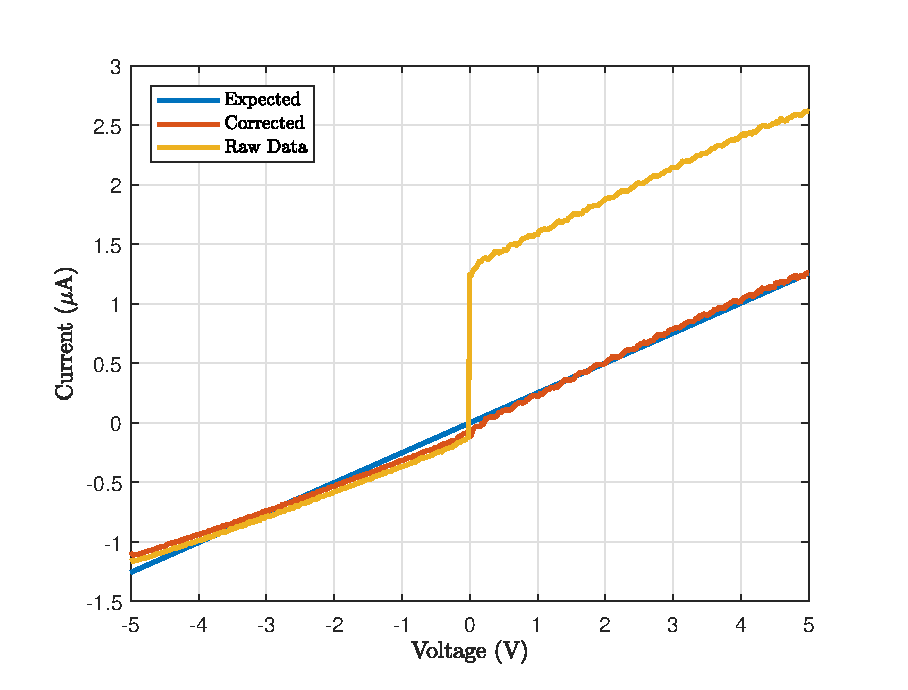
\includegraphics[width=\textwidth]{LP_plot_ohmic}
	\caption{The IV curve generated when a 3.98 M$\Omega$ resistor was placed across the probes. From the slope of the plot, the resistance is calculated to be $4.02$ M$\Omega$.}
	\label{fig:LP_plot_ohmic}
\end{figure}

It can be seen that there are small ripples in the current, which is a consequence of the smoothed PWM signal that was applied to the probes. By increasing the number of samples taken at each voltage value the magnitude of this ripple can be reduced. Lastly, the resistance is the inverse of the slope of this line, which was measured to be 4.02 M$\Omega$. This value is quite close to the measured value, which validates the ability of the circuitry to accurately measure current of the order $\mu$A.

\subsection{Further Testing}
As the capability to accurately measure micro amp current has been verified, the final testing required is a plasma environment test. The Langmuir probe will be connected to a micro-controller in a self contained system that is placed in a vacuum environment. A plasma will be established and multiple voltage sweeps will be performed and the data will be recorded. This data will be used to verify that the probes can obtain a correct IV curve. Furthermore, obtaining experimental data will allow for the data processing algorithm to be tested and validated. Once the data is obtained the algorithm can be refined, completing the design of the Langmuir probe.

\subsection{Probe Deployment Mechanism}
Two probes are required for the mission, where a single probe is a thin conducting metal rod that is extruded from the CubeSat into the plasma. For the real CubeSat, a thin rod of diameter 2 mm and length 60 mm is suitable for this purpose. However, as this will be need to be custom made, an `off the shelf' replacement will be used for the prototype in the form of a sewing needle. The probes are not required to point in any direction in order to function properly as the plasma is locally isotropic. The probes are constructed from stainless steel since the melting point is higher than the temperature of the ionosphere plasma. The probes are initially internal to the CubeSat, during launch and when the CubeSat is deployed. A mechanism has been designed which allows for the two probes to be extruded upon command. To assess possible solutions to this problem a trade off table (Table \ref{table:trade}) was used.\\

\begin{table}[]
\centering
\begin{tabular}{@{}lcccc@{}}
\toprule
                            & \textbf{Rack and Pinion} & \textbf{Bevel Gears} & \textbf{Spur Gears} & \textbf{Torsion Springs} \\ \midrule
Ease of Manufacture         & 3                               & 1                             & 4                          & 5                        \\
Reliability and Reusability & 5                               & 2                             & 4                          & 1                        \\
Weight and Size             & 1                               & 3                             & 3                          & 3                        \\
Displacement Allowed        & 5                               & 4                             & 4                          & 4                        \\
Electronic Requirements     & 1                               & 3                             & 3                          & 3                        \\
\textbf{Total}              & \textbf{15}                     & \textbf{13}                   & \textbf{18}                & \textbf{16}              \\ \bottomrule
\end{tabular}
\caption{Trade off table comparing proposed payload mechanisms}
\label{table:trade}
\end{table} 

The bevel gear system is clearly the worst design, using a central gear to rotate two smaller pinions that rotates the probes from a horizontal to vertical position along the $-z$ face of the MuirKat. Its issues stem from difficulties with manufacturing and design. The payload assembly was to be 3D printed using ABS and helical bevel gears were outside the scope of the capabilities of any printer available for this project, thus this design was rejected. The linear rack and pinion system was the only design to incorporate redundancy, involving two racks and two pinion gears that moved the probes linearly out along the $x$ direction through the use of a servo. However, since the Langmuir probes must come in pairs, even if one servo were to fail it makes no sense to deploy just one probe. Thus, despite containing mechanical redundancy, the unique requirements of the payload mean true redundancy would require four servo motors. This is reflected in the poor size/weight and electronic scores, leading to the rejection of this design. Lastly, rotary spur gears were selected over torsion springs, since the spur gears have comparable performance in all areas but are able to be used multiple times. The final payload assembly is shown in Figure \ref{fig:payload}. Note that that the torsion spring system still required electronics to operate in the form of a fuse wire that would be melted to release the spring energy and deploy the probes. In addition, although it is not listed in the table, the gear assemblies all perform better under vibration than the spring assembly since they don't have a natural tendency to displace under oscillation.\\

\begin{figure}[!h]
\centering 
\includegraphics[width=0.5\textwidth]{payload.JPG}
\caption{Computer render of the final payload assembly to be manufactured using 3D printed ABS (FDM process courtesy of Quang Vuong, chief of CS Sydney Solar)}
\label{fig:payload}
\end{figure}

The mechanism utilises a 50mm diameter spur gear at the centre, actuated by a sub-micro servo motor. The servo receives power from the battery and data from the OBC. Upon turning, two half-size (25 mm diameter) pinion gears are meshed at a 20$^{\circ}$ pressure angle. This rotation is put to work when the Langmuir probes are mounted on top. The probes `fan' out at 90$^{\circ}$ to the side of the MuirKat, anti-parallel to each other. This mechanism was the ideal solution for the MuirKat, meeting all the design requirements of the structural and payload subsystems whilst consuming little power and being simple to program.\\ 

In addition to housing the payload assembly, a secondary plate was added to make better use of the $z$ space occupied by the servo. Rather than waste this vertical distance, the second plate allows for the winding of the $z$ magnetorquer, cleaning up the satellite's assembly in the process.

\FloatBarrier
\newpage
\section{Structural Subsystem \label{structural}}

\subsection{Manufacturing and layout}
The finalised structure is represented in the computer render of figure \ref{ExplodedSat}. The external structure consists of 6061-T6 (space grade) Aluminium that has been CNC machined to within 0.1 mm maximum tolerance. Material properties for this structure are shown in table \ref{Materials}. The design itself is based on the ISIS structure, a flight proven commercial structure that has been quality tested for vibration, vacuum cycling, thermal cycling and stress. Assembly involves joining four ribs to two side frames using M3 bolted connections through countersunk un-threaded holes. Commercial GaAs solar panels and aluminium plates form the remainder of the external enclosure. \\
  
\begin{figure}[!h]
\centering	
\includegraphics[width=\textwidth]{ExplodedSat.JPG}
\caption{External exploded view of the MuirKat's final layout}
\label{ExplodedSat}
\end{figure}

The internal structure is custom to the MuirKat. The lower PCB contains the OBC and communications subsystems primary components, the middle PCB contains the ADCS and EPS subsystem, and the top two structures contain the payload PCB and deployment structure respectively. The PCBs themselves are glass fibre reinforced epoxy composites (FR4) with material properties as per those of table \ref{Materials}. The payload structure was manufactured using 3D printed (fused deposition modelling) ABS. The Langmuir probes are 2mm cold drawn stainless steel. \\ 

The assembly mechanism to connect the internal and external structures together involves steel spacers. These thread into each other, locking all the PCBs in place, then thread to the MuirKat structure itself. In organising the layout, heavier components were kept central in order to keep the centre of mass within the required 20 mm sphere (measured from geometric centre). Using SolidWorks the centre of mass is calculated as shown in table \ref{COM}. The value calculated is at most 6.89mm away from the geometric centre (50,50,50). In addition, the entire assembly conforms to the required directional launch standards as all PCBs align with the negative Z direction. 
  
\begin{table}[H]
\centering
\begin{tabular}{@{}lcccl@{}}
\toprule
                        & \textbf{6061-T6 Aluminium} & \textbf{FR4} & \textbf{ABS} & \textbf{Stainless Steel} \\ \midrule
  Young's Modulus (GPa) & 68.9                       & 21           & 2.5          & 193                      \\
  Density (kg/m$^{3}$)  & 2700                       & 1850         & 850          & 7700                     \\
 Poisson's Ratio       & 0.33                       & 0.118        & 0.35         & 0.30                     \\
 Yield Strength (MPa)  & 310                        & 70           & 40           & 215                      \\ \bottomrule
\end{tabular}
\caption{Material properties of core structural materials}
\label{Materials}
\end{table}
 
\begin{table}[]
\centering
\begin{tabular}{@{}lll@{}}
\toprule
\textbf{X (mm)} & \textbf{Y (mm)} & \textbf{Z (mm)} \\ \midrule
 49.89           & -46.98          & 56.11           \\ \bottomrule
\end{tabular}
\caption{Centre of Mass with frame of reference as illustrated in figure \ref{fig:COM}. The MuirKat satisfies QB50 requirements, keeping the COM within a 20 mm sphere from geometric centre}
\label{COM}
\end{table}
 
\begin{figure}
\centering	
\includegraphics[width=0.65\textwidth]{COM.PNG}
\caption{Centre of mass represented by the pink axes, reference coordinate system placed at the base of the side frame's top right corner}
\label{fig:COM}
\end{figure}
  
\begin{figure}
\centering	
\includegraphics[width=\textwidth]{coordinates}
\caption{Coordinate axes demonstrating - Z alignment of the MuirKat}
\end{figure}

\subsection{Mass Budget}
A detailed mass budget is attached in the appendix, a summary is represented here in table \ref{StrucBudget}. Approximately 60\% of the available mass was utilised. One might consider this under-design, however since the MuirKat successfully meets all the mission requirements as well as the QB50 mass requirements this is not a cause for concern. 
\begin{table}[!h]
\centering
\begin{tabular}{@{}lccc@{}}
\toprule
\textbf{}          & \textbf{}                     & \multicolumn{2}{c}{\textbf{Mass}}      \\ \midrule
\textbf{Subsystem} & \textbf{Number of Components} & \textbf{Mass}   & \textbf{Contingency} \\
OBC                & 12                            & 107.50          & 10.75                \\
EPS                & 6                             & 47.70           & 2.12                 \\
TTC                & 12                            & 29.40           & 2.51                 \\
Payload            & 17                            & 18.14           & 4.60                 \\
ADCS               & 22                            & 143.51          & 37.00                \\
Structure          & 9                             & 213.21          & 21.00                \\
Thermal            & 1                             & 50.00           & 0.10                 \\
\textbf{Total}     & \textbf{79}                   & \textbf{609.46} & \textbf{687.54}      \\ \bottomrule
\end{tabular}
\caption{Summary Mass Budget}
\label{StrucBudget}
\end{table}

\subsection{Simulation Method}
To perform finite element analysis a simulation criterion is required. All simulations consider a typical CubeSat launch such as those from a P-Pod launcher or NanoRack system. This involve keeping the negative Z face fixed, but allowing the positive Z face to have a small displacement. This displacement arises due to the kill switch not being rigidly fixed when in contact with the launch armature. The frame itself is also not a rigid structure, relying on M3 bolts to join all elements. To simulate this, all contacts between the frames and ribs were suppressed. A typical P-Pod launch structure is shown in figure \ref{fig:P-Pod}. 
  
 \begin{figure}[H]
 \centering	
 \includegraphics[width=0.5\textwidth]{P-Pod.jpg}
 \caption{Illustration of a typical P-Pod launch system for CubeSat deployment. Available at \text{http://www.pe0sat.vgnet.nl/wp-content/uploads/2011/11/P-Pod-Launcher.jpg} [Accessed October 29 2017]}
 \label{fig:P-Pod}
 \end{figure}
 
% Modes 
\subsection{Modal Analysis}
The modal analysis produced interesting results, highlighting the structural weakness that is the Langmuir probe. The first 5 modes at three mesh sizes are shown in table \ref{table:modes}. The solution appears to begin to converge for lower modes (expected 240-245 Hz convergence point), however the higher modes still demonstrate a level of uncertainty. Unfortunately the finest mesh (3 mm) was the computing limit of the hardware available for this project and so we settle for the results in table \ref{table:modes}. \\

\begin{table}[]
\centering
\begin{tabular}{@{}lccccc@{}}
\toprule
\multicolumn{1}{c}{\textbf{Element Size (mm)}} & \textbf{Mode 1 (Hz)} & \textbf{Mode 2 (Hz)} & \textbf{Mode 3 (Hz)} & \textbf{Mode 4 (Hz)} & \textbf{Mode 5 (Hz)} \\ \midrule
10                                             & 253.34               & 254.41               & 255.72               & 258.42               & 393.64               \\
5                                              & 253.29               & 253.73               & 254.43               & 257.41               & 350.75               \\
3                                              & 247.03               & 249.11               & 249.32               & 250.49               & 354.98               \\ \bottomrule
\end{tabular}\caption{Results of Modal Analysis}
\label{table:modes}
\end{table} 

The first 4 modes provide the most interesting discussion due to their close spacing. Observing figure \ref{fig:mode1} we account for this by reasoning the Langmuir probes acts as an elastic beam. Keeping the probes free at one end means they have poor vibration performance, noticeable by observing how the 5th mode (the first due to the structure alone, as shown in figure \ref{fig:mode5}) is approximately 100 Hz away from the first mode due to the langmuir probes. If the probes were to be fixed we would expect to achieve a 100 Hz improvement in vibration performance. However, this we would lose all the benefits of the spur gear payload mechanism and instead return to what was expected of a torsion spring system. As such the decision to keep the payload structure as it stands was preferred, primarily due to the fact that the fundamental mode is still well above the 90 Hz requirement (QB50). 

\begin{figure}[H]
\centering	
\includegraphics[width=\textwidth]{mode1}
\caption{Simulation result of the first mode at finest mesh (247.03 Hz). The Langmuir probes acts as elastic beams and prove a considerable weakpoint within the structure. Scale in units 1e-3 meters, i.e max deflection 3.8 mm}
\label{fig:mode1}
\end{figure}

\begin{figure}[H]
\centering	
\includegraphics[width=\textwidth]{mode5}
\caption{Simulation result for the fifth mode at finest mesh (354.98 Hz). This is the first mode due to the structure as a whole instead of the Langmuir probes}
\label{fig:mode5}
\end{figure}


% Acceleration 
\subsection{Quasistatic Acceleration Analysis}

With the simulation method remained unchanged a constant acceleration load of 10.8g was applied along each coordinate axes as per QB50 requirements. The results for the three cases are summarised in table \ref{table:stresses}. \\ 

\begin{table}[]
\centering
\begin{tabular}{@{}lccc@{}}
\toprule
\textbf{Element Size (mm)} & \multicolumn{1}{l}{\textbf{Max Stress X (MPa)}} & \multicolumn{1}{l}{\textbf{Max Stress Y (MPa)}} & \multicolumn{1}{l}{\textbf{Max Stress Z (MPa)}} \\ \midrule
10                         & 20.6                                            & 32.8                                            & 7.3                                             \\
5                          & 23.8                                            & 33.5                                            & 7.6                                             \\
3                          & 24.2                                           & 34.1                                             & 7.6                                             \\ \bottomrule
\end{tabular}
\caption{Maximum stress values calculated using FEA under 10.8g acceleration load}
\label{table:stresses}
\end{table}

The maximum stress listed uses the Von-Mises energy method of calculation. This is considered the best indication of yielding behaviour. Using table \ref{Materials} we see that no component will experience a stress larger than it's yield value. The weakest structural element is the ABS plastic used in the payload at 40 MPa. The largest maximum stress occurs along the Y direction, appearing to converge at 35 MPa. This indicates a factor of safety of 1.15, a relatively tight tolerance. If the satellite was given a longer development cycle the payload would be re-made using better materials (preferably the same FR4 composite for the base and aluminium for the gears), this would raise the factor of safety to 1.75. \\

In addition to these stress values, the total deformation of the structure is a useful visualisation tool. Figures \ref{fig:defX}, \ref{fig:defX} and \ref{fig:defX} explicitly demonstrate how the cubesat deforms inside the P-Pod. All values are on the order $1\times 10^{-5} \ \text{m}$ and the MuirKat is considered space-ready from a structural standpoint. 

\begin{figure}[H]
\centering	
\includegraphics[width=\textwidth]{deformationX}
\caption{Total deformation of the MuirKat in the X direction. Along the X axis the deformation is distributed primarily throughout the internal structure, as supported by the equivalent stress value that lies between the maximum and minimum values seen along all axis.}
\label{fig:defX}
\end{figure}

\begin{figure}[H]
\centering	
\includegraphics[width=\textwidth]{deformationY}
\caption{Total deformation of the MuirKat in the Y direction. The Y direction contained the highest stress and deformation figures, this is due to the fact they the acceleration occurs in the same direction as the resonant deflection of the Langmuir probes. Again, leaving these probes free proved to be a considerable weak point within the structure.}
\label{fig:defY}
\end{figure}

\begin{figure}[H]
\centering	
\includegraphics[width=\textwidth]{deformationZ}
\caption{Total deformation of the MuirKat in the Z direction. This axis did not see large values of stress or deformation, attributed to the fact that both Aluminium and FR4 are strong in compression. Noticeably the ABS plastic (and of course the probes) are the weak elements in this coordinate direciton.}
\label{fig:defZ}
\end{figure}
 
\FloatBarrier
\newpage
\begin{appendix}
	\section{Code}
\subsection{Payload} \label{app:code_payload}
The follow code contains functions used by the OBC to perform the voltage sweep and analyse the data.

\lstinputlisting[style=CStyle]{code/payload/LP_functions.ino}

\subsection{Attitude Determination and Control \label{app:mat}}

\subsubsection{Main code}

\lstinputlisting{code/adcs/main_display.m}

\subsubsection{Satellite Dynamics: \texttt{satDyn.m}}

\lstinputlisting{code/adcs/satDyn.m}

\subsubsection{ADCS Loop: \texttt{adcs.m}}

\lstinputlisting{code/adcs/adcs.m}

\subsubsection{Unscented Kalman Filter: \texttt{UKF.m}}

\lstinputlisting{code/adcs/UKF.m}

\subsubsection{Controllers: \texttt{controlLQR.m}}

\lstinputlisting{code/adcs/controlLQR.m}

\section{Link Calculations \label{app:LinkCalc}}
The following values are typical for this type of system, and have been derived from research: bit error rate $<10^-5$, LNA noise temperature $T_{down}=50K, T_{up}=289K$, spacecraft transmission line temperature $T_{trans, sat} = 51.2K$ demodulation implementation loss $3dB$, threshold $E_{b}/N_{0}=9.6dB$ \cite{SMAD}, ground station transmission line loss $3.29dB$ \cite{LineLossGS}, loss due to rain/snow $0dB$, ionospheric loss $0.1dB$ \cite{RainLoss}, atmospheric loss $1dB$ \cite{AtmosLoss}, transponder intermodulation ratio $IMR=50dB$, per used channel bandwidth $BW_{user}=air data rate/2=4kbps$, spacecraft sky temperature $T_{sky, down}=90K$, $T_{sky, up}=290K$ \cite{SMAD}, antenna polarisation loss $L_{pol}=-3dB$ and the transponder uplink interference density $\rho_{int, up}=-250dbW/Hz$.

\subsection{Slant Range}
The slant range is the measure of the maximum distance between the satellite and the groundstation, and will be used to later find the free-space loss.
It can simply be found using geometry, the elevation angle of the satellite and it's altitude. The altitude for the chosen orbit is $400$km, and the elevation angle is $35^o$. We need a minimum of $20^o$ to be visible by the earth at all, to which we add the $5^o$ for visibility.
\begin{equation}
slant range = \dfrac{altitude}{sin(\theta_{el})}=697.38km
\end{equation}

\subsection{Pointing Loss}
The pointing loss is loss associated with the antenna of the satellite not being accurately pointed at the ground station and vice versa. Due to the high velocity of the satellites this is easily possible, and they can be found using the following formula.
\begin{equation}
pointing loss = \frac{12\alpha_{T}}{\theta_{3dB}}=1dB_{Dipole}, 3dB_{Yagi}
\end{equation}
Where the angle of misalignment has been chosen to be $\alpha_{T}=8.4^o$, and the $\theta_{3dB}$, the beam width at half power is $80^o$ and $50^o$ \cite{BeamWidth} for the dipole and the yagi-type antenna respectively.

\begin{landscape}
		\clearpage\pagestyle{empty} 
\subsection{Power Budget}
	\begin{figure}[H]
		\centering
		\includegraphics[scale=0.8]{power_budget}
		\caption{Power budget}
		\label{fig_pwrBud}
	\end{figure}
\end{landscape}

\subsection{EIRP}
The effective isotropic radiated power is a simple measure of an antennas radiated power, by assuming it's an isotropic radiator\cite{SMAD}.
This measure can be found by adding the transmitter power, with the antenna gain and taking away the transmission line losses, when working in dB.
\begin{equation}
EIRP=P_{T}+G_{A}-L_{T}
\end{equation}

\subsection{Free Space Loss}
The free space loss is the largest part of the power loss, and it occurs over the distance the signal has to travel through free space. It is calculated the following formula, where $R$ is the slant range, $f$ is the frequency of transmission in Hz, and $c$ is the speed of light.

\begin{equation}
FSPL=(\frac{4\pi Rf}{c})^2
\end{equation}

\subsection{Figure of Merit}
Figure of merit is a measure of how the gain of the antenna compares to the noise in the system. It can be found using the gain of the antenna $G_{A}$ and the system noise temperature $T_{s}$, both in decibels.
\begin{equation}
FoM=G_{A}-T_{s}
\end{equation}

\subsection{Carrier Power}
The carrier power is a measure of the energy of the carrier signal. This means it is simply the sum of all gains and losses with the EIRP.

\begin{equation}
C=EIRP+G-L
\end{equation}

\subsection{Noise Density}
As we can see the carrier power is relatively small, but due to the system set-up, so is the noise density. This can be found by converting the noise temperature to an amplitude in decibels, using Boltzmann's constant.

\begin{equation}
N_0=k_{b, dB}+T_{s}
\end{equation}

\subsection{Carrier Power to Noise Density Ratio}
This ratio is relatively self-explanatory, as it expresses the ratio between the strength of the signal to the noise present. It can be found using
\begin{equation}
C-N ratio=\dfrac{C}{N_{0}}
\end{equation}


\subsection{$E_{b}/N_{0}$}
This measure is closely related to the C-N ratio, but instead of the total power it gives the energy per bit, compared to the noise density. To get this value, we simply need to divide by the data-rate $R_b$ chosen.
\begin{equation}
E_{b}/N_{0}=\frac{C}{N_{0}}-10\log(R_b)=20.02dB_{up}, 16.75dB_{down}
\end{equation}

The combined ratio is given to be $15.07dB$. Every modulation technique has a threshold value, under which the noise will be too large to decipher the original signal. For the chosen method this limit is $9.6dB$.\\

This then leaves a system link margin of $10.42dB$ for uplink and $7.15dB$ for downlink in the link performance.

\section{Detailed Mass Budget}

\begin{landscape}
	\clearpage\pagestyle{empty} 
	\begin{figure}[H]
		\centering
		\includegraphics[scale=0.7]{MassBudgie}
		\caption{Mass Budget}
		\label{MassBudgie}
	\end{figure}
\end{landscape}

\end{appendix}
\FloatBarrier
\newpage

\bibliography{references}
\bibliographystyle{unsrt}

\pagebreak

\end{document}